

\section{Πρόσθεση στο Δυαδικό}
Οι αριθμητικές πράξεις με αριθμούς αναπαράστασης συγκεκριμένης βάσης ακολουθούν τους ίδιους κανόνες
με αυτούς του δεκαδικού συστήματος, χρησιμοποιώντας σε κάθε περίπτωση μόνο τα διαθέσιμα ψηφία ανάλογα την βάση. Στα πλαίσια αυτής της διπλωματικής χρησιμοποιείται το δυαδικό σύστημα εφόσον κύριο θέμα 
της είναι η επιτάχυνση των δυαδικών αθροιστών υπολοίπου.





\subsection{Πρόσθεση δύο ψηφίων}
Στην πρόσθεση δύο δυαδικών ψηφίων $x+y$ υπάρχουν τέσσερις πιθανές περιπτώσεις σύμφωνα με το συνδυασμό
των τιμών που παίρνει το κάθε ψηφίο (0 ή 1). Στην περίπτωση $0+0$ το αποτέλεσμα είναι προφανώς μηδέν 
και ίδιο με εκείνο του δεκαδικού συστήματος. Οι περιπτώσεις $0+1$ και $1+0$ έχουν κοινό αποτέλεσμα, 
ίσο με ένα και αυτό οφείλεται στην προσεταιριστική ιδιότητα της πρόσθεσης, η οποία ισχύει σε όλα
τα αριθμητικά συστήματα. Τελευταία περίπτωση είναι και η πιο περίπλοκη, όπου $1+1$ έχει άθροισμα μηδέν
και ένα κρατούμενο. Στον πίνακα \ref{tb:HA_truth_table} παρουσιάζεται ο πίνακας αληθείας, δηλαδή ο 
πίνακας που περιγράφει την συμπεριφορά των εξόδων, στην περίπτωση αυτή το άθροισμα (sum) και το 
κρατούμενο ($c_{out}$), σύμφωνα με κάθε πιθανό συνδυασμό των εισόδων x και y.


\begin{multicols}{2}
% Table Half Adder
%------------------------------------------
\hfill
\begin{table}[H]
\centering
 \begin{tabular}{||c c | c c||} 
 \hline
 x & y & sum & $c_{out}$ \\ [0.5ex] 
 \hline\hline
 0 & 0 & 0 & 0 \\ 
 \hline
 0 & 1 & 1 & 0 \\
 \hline
 1 & 0 & 1 & 0 \\
 \hline
 1 & 1 & 0 & 1 \\
 \hline
\end{tabular}
\caption{Πίνακας αληθείας ημιαθροιστή}
 \label{tb:HA_truth_table}
\end{table}


% Figure
% HA-Schematic
%--------------------------------------------
\begin{figure}[H]
\centering
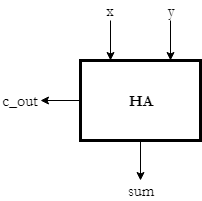
\includegraphics[scale=0.6]{HA.png}
\caption{Σύμβολο ημιαθροιστή}
\label{HASchematic}
\end{figure}

\end{multicols}

Το παραπάνω σύστημα ονομάζεται ημιαθροιστής ή Half-Adder (HA) , έχει δυο εισόδους τις x και y και δυο εξόδους τις $c_{out}$ και sum και οι έξοδοι σύμφωνα με τον πίνακα αληθείας περιγράφονται από τις παρακάτω συναρτήσεις άλγεβρας Boole, όπου με $+$ συμβολίζεται η λογική πράξη ΟR, με $*$ η λογική πράξη ΑΝD , με $!$ η λογική αντιστροφή INVERT και με $\oplus$ η λογική πράξη XOR :\\
\begin{equation}
\begin{split}
    sum &= x \oplus y \\ 
    c_{out} &= x * y
\end{split}
\end{equation}\\



Από τον ημιαθροιστή δομείται ο πλήρης αθροιστής ή Full-Adder (FA) με τρεις εισόδους x, y, z , δυο εξόδους sum και $c_{out}$ και λειτουργία αντίστοιχη του FA με την διαφορά πως ο FA προσθέτει τρία δυαδικά ψηφιά \\
\begin{multicols}{2}
\hfill
\begin{table}[H]
\centering
 \begin{tabular}{||c c c | c c||} 
 \hline
 x & y & z & sum & $c_{out}$ \\ [0.5ex] 
 \hline\hline
 0 & 0 & 0 & 0 & 0 \\ 
 \hline
 0 & 0 & 1 & 1 & 0 \\
 \hline
 0 & 1 & 0 & 1 & 0 \\
 \hline
 0 & 1 & 1 & 0 & 1 \\
 \hline
 1 & 0 & 0 & 1 & 0 \\ 
 \hline
 1 & 0 & 1 & 0 & 1 \\
 \hline
 1 & 1 & 0 & 0 & 1 \\
 \hline
 1 & 1 & 1 & 1 & 1 \\
 \hline
\end{tabular}
\caption{Πίνακας αληθείας πλήρη αθροιστή}
\label{table:2}
\end{table}
% Figure
% FA-Schematic
%--------------------------------------------
\begin{figure}[H]
\centering
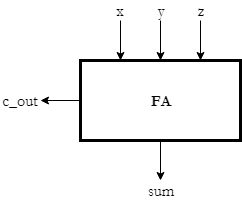
\includegraphics[scale=0.3]{FA.png}
\caption{Σύμβολο πλήρη αθροιστή}
\label{FASchematic}
\end{figure}
\end{multicols}
και οι εξισώσεις των εξόδων είναι :
\begin{equation}
\begin{split}
    sum &= x \oplus y \oplus z \\
    c_{out} &= ( x * y ) + ( x * z ) + ( z * y )
\end{split}
\end{equation}




% 
%------------------------------------------------------------
\subsection{Πρόσθεση δυαδικών αριθμών}

Η πρόσθεση δυο δυαδικών αριθμών A και Β των n δυαδικών ψηφίων είναι 
μια επέκταση της πρόσθεσης μεταξύ ψηφίων που παρουσιάστηκε προηγουμένως τροφοδοτώντας 
το κρατούμενο εξόδου των προηγούμενων σημαντικών ψηφίων στην είσοδο του πλήρη αθροιστή 
των επομένων. Το $c_{i}$ συμβολίζει το κρατούμενο που παράγεται από την πρόσθεση των ψηφίων 
$a_i+b_i$. Επομένως το κάθε ψηφίο αθροίσματος, υπολογίζεται από την 
λογική συνάρτηση:
\begin{equation}
    sum_i = a_i \oplus b_i \oplus c_{i-1}\\
\end{equation}
Πρέπει να σημειωθεί πως στο $sum_0 = a_0 \oplus b_0 \oplus c_{-1}$, το $c_{-1}$ έιναι το κρατούμενο εισόδου του αθροιστή (αν υπάρχει).
% Figure
% FA-Schematic
%--------------------------------------------
\begin{figure}[H]
    \centering
    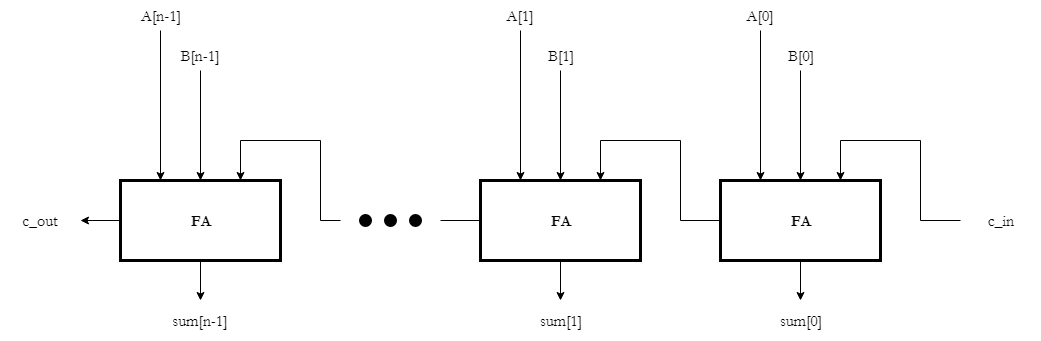
\includegraphics[width=\textwidth]{IntAdder.png}
    \caption{Απλός αθροιστής διάδοσης κρατουμένου}
    \label{IntegerAdderSchematic}
\end{figure}
Ο αθροιστής στην εικόνα \ref{IntegerAdderSchematic} αποτελεί τον πιο κλασικό σχεδιασμό 
με αρκετά μικρή επιφάνεια και κατανάλωση ενέργειας αλλά πολύ υψηλούς χρόνους καθυστέρησης 
για τον υπολογισμό του αθροίσματος. Με κόκκινη γραμμή συμβολίζεται το κρίσιμο μονοπάτι. Είναι εμφανές πως για τον υπολογισμό του σημαντικότερου ψηφίου του αθροίσματος είναι αναγκαίο να έχουν οριστικοποιηθεί οι έξοδοι όλων των προηγούμενων στοιχείων άθροισης. Στην συνέχεια θα παρουσιαστούν μέθοδοι εξάλειψης του φαινομένου αυτού με διάφορες τεχνικές.



